%   DOCUMENT CLASS  %%%%%%%%%%%%%%%%%%%%%%%%%%%%%%%%%%%%%%%%%%%%%%%%%%%%%%%%%%%
%
%   Use the `sfuthesis` class to format your thesis.
%
%   For more information about thesis formatting requirements, go to
%   http://www.lib.sfu.ca/help/publish/thesis or ask a thesis advisor at the
%   SFU Research Commons.


\documentclass{sfuthesis}



%   DOCUMENT METADATA  %%%%%%%%%%%%%%%%%%%%%%%%%%%%%%%%%%%%%%%%%%%%%%%%%%%%%%%%
%
%   Fill in the following information for the title page and declaration of
%   committee page. Please review the Declaration of Committee page
%   instructions on the library's thesis website before completing this page:
%   https://www.lib.sfu.ca/help/publish/thesis/format/declaration-committee

%   Choose the \faculty entry below from the following list:
%
%       - Faculty of Applied Sciences
%       - Faculty of Arts and Social Sciences
%       - Beedie School of Business
%       - Faculty of Communication, Art and Technology
%       - Faculty of Education
%       - Faculty of Environment
%       - Faculty of Health Sciences
%       - Faculty of Science

\title{Computational strategies for the nonlinear elastodynamics of skeletal muscle tissue}
\thesistype{Thesis}
\author{Javier Alejandro Almonacid Paredes}
\previousdegrees{%
    M.Sc., Simon Fraser University, 2020\\
    B.Sc., Universidad de Concepci\'{o}n, 2015}
\degree{Doctor of Philosophy}
\department{Department of Mathematics}
\faculty{Faculty of Science}
\copyrightyear{2025}
\semester{Spring 2025}


%   You may include up to six keywords or phrases. Keywords should be separated
%   with semicolons. No punctuation at the end.
\keywords{thesis template; Simon Fraser University; \LaTeX; time travel paradoxes}

\committee{
    \chair{TBD}{Professor \\ Department of Mathematics}
    \member{Nilima Nigam}{Supervisor \\ Professor \\ Department of Mathematics}
    \member{James Wakeling}{Committee Member (?)\\ Professor \\ Department of Biomedical Physiology and Kinesiology}
    \member{TBD}{Internal Examiner \\ Professor \\ Department of Mathematics}
    \member{TBD}{External Examiner \\ Professor \\ Department of Quantum Fields \\ Mars University}
}



%   PACKAGES %%%%%%%%%%%%%%%%%%%%%%%%%%%%%%%%%%%%%%%%%%%%%%%%%%%%%%%%%%%%%%%%%%
%
%   Add any packages you need for your thesis here.
%   You don't need to call the following packages, which are already called in
%   the sfuthesis class file:
%
%   - appendix
%   - etoolbox
%   - fontenc
%   - geometry
%   - lmodern
%   - nowidow
%   - setspace
%   - tocloft
%
%   If you call one of the above packages (or one of their dependencies) with
%   options, you may get a "Option clash" LaTeX error. If you get this error,
%   you can fix it by removing your copy of \usepackage and passing the options
%   you need by adding
%
%       \PassOptionsToPackage{<options>}{<package>}
%
%   before \documentclass{sfuthesis}.
%
%   The following packages are a few suggestions you might find useful.
%
%   (1) amsmath and amssymb are essential if you have math in your thesis;
%       they provide useful commands like ``blackboard bold'' symbols and
%       environments for aligning equations.
%   (2) amsthm includes allows you to easily change the style and numbering of
%       theorems. It also provides an environment for proofs.
%   (3) graphicx allows you to add images with \includegraphics{filename}.
%   (4) hyperref turns your citations and cross-references into clickable
%       links, and adds metadata to the compiled PDF.
%   (5) pdfpages lets you import pages of external PDFs using the command
%       \includepdf{filename}. You will need to do this if your research
%       requires an Ethics Statement.
%

\usepackage{amsmath}                            % (1)
\usepackage{amssymb}                            % (1)
\usepackage{amsthm}                             % (2)
\usepackage{graphicx}                           % (3)
\graphicspath{{figs/}}
\usepackage{epstopdf}
\usepackage[pdfborder={0 0 0}]{hyperref}        % (4)
% \usepackage{pdfpages}                         % (5)
% ...
% ...
% ...
% ... add your own packages here!

\usepackage{background}
\backgroundsetup{
  position=current page.north,
  angle=0,
  nodeanchor=north,
  vshift=-10mm,
  opacity=1,
  scale=1.5,
  contents=Submitted for revision on \today
}

\usepackage{circuitikz}
\usetikzlibrary{patterns,hobby,decorations.pathmorphing}


%   OTHER CUSTOMIZATIONS %%%%%%%%%%%%%%%%%%%%%%%%%%%%%%%%%%%%%%%%%%%%%%%%%%%%%%
%
%   Add any packages you need for your thesis here. We've started you off with
%   a few suggestions.
%
%   (1) Use a single word space between sentences. If you disable this, you
%       will have to manually control spacing around abbreviations.
%   (2) Correct the capitalization of "Chapter" and "Section" if you use the
%       \autoref macro from the `hyperref` package.
%   (3) The LaTeX thesis template defaults to one-and-a-half line spacing. If
%       your supervisor prefers double-spacing, you can redefine the
%       \defaultspacing command.
%

\frenchspacing                                    % (1)
\renewcommand*{\chapterautorefname}{Chapter}      % (2)
\renewcommand*{\sectionautorefname}{Section}      % (2)
\renewcommand*{\subsectionautorefname}{Section}   % (2)
% \renewcommand{\defaultspacing}{\doublespacing}  % (3)
% ...
% ...
% ...
% ... add your own customizations here!

\usepackage{bm,bbm}
\usepackage{empheq}

%-----------------------------------------------
% Eliminate ugly boxes around references.
\usepackage{xcolor}
\hypersetup{
    colorlinks,
    linkcolor={red!50!black},
    citecolor={blue!50!black},
    urlcolor={blue!80!black}
}
%------------------------------------------------

\numberwithin{equation}{chapter}
\numberwithin{figure}{chapter}
\numberwithin{table}{chapter}


\newtheorem{objective}{Objective}
\renewcommand*{\theobjective}{\Alph{objective}}
\newtheorem{theorem}{Theorem}[chapter]
\newtheorem{remark}[theorem]{Remark}

\theoremstyle{definition}
\newtheorem{definition}{Definition}[chapter]
\newtheorem{lemma}[definition]{Lemma}
\newtheorem{example}[definition]{Example}

%%%%%%%%%%%%%%%%%%%%%%%%%%%%%%%%%%%%%%%%%%%%%%%%%%%
%
%  DEFINITIONS 
%
%%%%%%%%%%%%%%%%%%%%%%%%%%%%%%%%%%%%%%%%%%%%%%%%%%%

\def\*#1{{\mathbf{#1}}} % bold letters!
\newcommand{\pder}[2]{\dfrac{\partial #1}{\partial #2}}
\newcommand{\Dder}[2]{\dfrac{\mathrm{D} #1}{\mathrm{D} #2}}
\newcommand{\der}[2]{\dfrac{\mathrm{d} #1}{\mathrm{d} #2}}
\newcommand{\dder}[2]{\dfrac{\mathrm{d} #1}{\mathrm{d} #2}}
\newcommand{\divs}[1]{{\mathrm{div} \, #1}}
\newcommand{\Divs}[1]{{\mathrm{Div} \, #1}}
\newcommand{\divt}[1]{{\bm{\mathrm{div}} \, #1}}
\newcommand{\Divt}[1]{{\bm{\mathrm{Div}} \, #1}}

\newcommand{\depsilon}{\dot{\varepsilon}}
\newcommand{\R}{\mathbb{R}}
\newcommand{\B}{\mathcal{B}}
\newcommand{\F}{\mathcal{F}}
\newcommand{\I}{{\bar{I}}}
\newcommand{\FF}{{\bm{\mathcal{F}}}}
\newcommand{\C}{\mathbb{C}}
\newcommand{\T}{\top}
\renewcommand{\c}{\mathbbm{c}}
\renewcommand{\P}{\mathbb{P}}
\newcommand{\p}{\mathbbm{p}}
\newcommand{\vphi}{\varphi}

\def\bsigma{{\bm{\sigma}}}
\def\btau{{\bm{\tau}}}
\def\bchi{{\bm{\chi}}}
\def\bxi{{\bm{\xi}}}
\def\bphi{{\bm{\varphi}}}

\newcommand{\javicomment}[1]{\noindent {\color{red}\textbf{Comment by Javi: #1}}}

%%%%%%%%%%%%%%%%%%%%%%%%%%%%%%%%%%%%%%%%%%%%%%%%%%%
%
% END OF DEFINITIONS
%
%%%%%%%%%%%%%%%%%%%%%%%%%%%%%%%%%%%%%%%%%%%%%%%%%%%



%   FRONTMATTER  %%%%%%%%%%%%%%%%%%%%%%%%%%%%%%%%%%%%%%%%%%%%%%%%%%%%%%%%%%%%%%
%
%   Title page, committee page, abstract, dedication, acknowledgements, table
%   of contents, etc.
%
%   If your research requires an Ethics Statement, download the pdf from
%   https://www.lib.sfu.ca/help/publish/thesis/regulations#ethics-statement
%   to your thesis folder, then uncomment the appropriate lines below.

\begin{document}

\frontmatter
\maketitle{}
\makecommittee{}

%\addtoToC{Ethics Statement}%
%\includepdf[pagecommand={\thispagestyle{plain}}]{ethics_statement_piii.pdf}%
%\clearpage

\begin{abstract}
Abstract paragraphs should be unindented. Master's abstracts are limited to 150 words; the limit is 350 words for doctoral abstracts. Abstract text must fit on a single page.
\end{abstract}


\begin{dedication}
This is an optional page. Use your choice of paragraph style for text on this page.
\end{dedication}


\begin{acknowledgements}
This is an optional page. Use your choice of paragraph style for text on this page.
\end{acknowledgements}

\addtoToC{Table of Contents}%
\hypersetup{linkbordercolor=black,hidelinks}
\tableofcontents%
\clearpage

%   This is an optional page. Remove the following lines if you don't have any tables.
\addtoToC{List of Tables}%
\listoftables%
\clearpage

%   This is an optional page. Remove the following lines if you don't have any figures.
\addtoToC{List of Figures}%
\listoffigures%
\clearpage





%   MAIN MATTER  %%%%%%%%%%%%%%%%%%%%%%%%%%%%%%%%%%%%%%%%%%%%%%%%%%%%%%%%%%%%%%
%
%   Start writing your thesis --- or start \include ing chapters --- here.
%

\mainmatter%

\chapter{Introduction}

Start writing or pasting in your text here. By default, only works cited in the text will be added to the bibliography~\cite{HolzapfelBook}.

\section{Physiology of skeletal muscle}

\section{State of the art in muscle modelling}

\section{Continuum mechanics of deformable solids}

This might be a long section, maybe could be a chapter at the beginning of part 2? Should include some comments on generic deformation $\rho_0 \*u_{tt} = \Divt{\*P} + \*f$ and reduction to 1D if this is left as a section in the Introduction.

\part{One-dimensional elastodynamics}

\chapter{Inertial effects in multi-body mass-spring models of the muscle-tendon unit}

Work with Evan on mass enhanced muscle models. We need to discuss what would be appropriate to show here, besides the model and the numerical strategy (dynamic/mass effects? Focus on one cycle? Effects of different muscles and activities?).
Github repository: mass-enhanced-muscle-models.

\medskip

Things that are not in Evan's thesis:
\begin{enumerate}
    \item tendon dynamics
    \item what happens as the number of masses increases (homogenization study)
\end{enumerate}

Understanding the elastodynamics of skeletal muscle requires us to have an idea on the expected behaviour of muscle models. As a first approach to this task, we consider one-dimensional actuators. These are models that are well-established in the literature and that are part of major biomechanics software, such as OpenSim and FEBio [REFS]. Despite their apparent simplicity, however, these models are typically made of one or more highly-nonlinear ODEs whose stiff character cannot be overlooked. 

\hrulefill

\section{Mathematical description}

Consider the dynamic contraction of a muscle-tendon unit of length $L = L(t)$. Moreover, let $L_M$ and $L_T$ denote the muscle and tendon lengths, respectively, which satisfy $L_M(t) + L_T(t) = L(t)$ at every time $t \geq 0$.

We first define the \textit{muscle stretch} $\lambda_M$, the \textit{muscle strain} $\varepsilon_M$, and the {strain rate} $\depsilon_M$ as
\begin{equation}
    \lambda_M := \dfrac{L_M}{l_{mus}^{opt}}, \qquad \varepsilon_M := \lambda_M - 1, \qquad \depsilon_M = \dfrac{1}{\depsilon_0} \dder{\lambda_M}{t} = \dfrac{1}{l_{mus}^{opt} \, \depsilon_0} \dder{L_M}{t},
\end{equation}
where $l_{mus}^{opt}$ is the optimal muscle length and $\depsilon_0$ is the maximum unloaded shortening strain rate. Similarly, we define the \textit{tendon stretch} $\lambda_T$ and \textit{tendon strain} $\varepsilon_T$ as
\begin{equation}
    \lambda_T := \dfrac{L_T}{l^{opt}_{ten}}, \qquad \varepsilon_T := \lambda_T - 1,
\end{equation} 
with $l_{ten}^{opt} = L(0) - l_{mus}^{opt}$ being the optimal tendon length. The optimal muscle and tendon length corresponds to the length of the muscle and tendon parts of the MTU, respectively, at which the (relaxed) muscle is in static equilibrium.  These values can be initially calculated from literature, however, because we will be dealing with experimental data, some calibration is needed to ensure simulations begin from dynamic equilibrium (see Appendix \ref{app:calibration_optimal_initial_values}).

In a simple model, such as the one shown in Figure \ref{fig:muscle_models_1D}A, muscle can be thought as a one-dimensional spring containing a contractile element (CE) and a parallel elastic element (PEE). The first one is related to the force produced by actin-myosin interactions during activation, whereas the latter is related to passive components of the muscle fibre (such as titin), which act to prevent overstretching of the sarcomeres that form the muscle fibre. The muscle force $F_M$ in this case is given by Hill's equation,
\begin{equation} \label{eq:Hill_force}
    F_{Hill}(\lambda, \depsilon) = F_0 \Big\{ a(t) F_A(\lambda) F_V(\depsilon) + F_P(\lambda) \Big\}.
\end{equation}
Several components can be identified in this equation:
\begin{enumerate}
    \item $F_0$ is the maximum isometric force that the muscle in study can exert on the tendon,
    \item $a = a(t)$ is an activation function characterizing the influx of $\mathrm{Ca}_2^+$ ions that trigger the formation of cross-bridges between actins and myosins within sacomeres. This function can be computed given an excitation $u(t)$ using Zajac's equation \cite{Zajac1989}:
    \begin{equation}
        \dfrac{da}{dt} + \dfrac{a(t)}{\tau_{act}} \left( \beta + (1-\beta)u(t) \right) = \dfrac{u(t)}{\tau_{act}},
    \end{equation}
    \item $F_A = F_A(\lambda)$ is the active force-length relationship, 
    \item $F_V = F_V(\depsilon)$ is the force-velocity relationship, 
    \item $F_P = F_P(\lambda)$ is the passive force-length relationship.
\end{enumerate} 
The force relationships $F_A$, $F_V$, and $F_P$ are typically fit from experimental data obtained through tensile experiments, and therefore do not have a standard expression. For this particular set of experiments, we use least-squares fits of the B\'{e}zier curves used by Ross et. al [CITATION]. The exact definition of these curves is available in Appendix B. Moreover, the muscle force $F_M$ is balanced by the tendon force $F_T$ at all times, that is
\begin{equation} \label{eq:massless_model}
    F_M(\lambda_M, \depsilon_M) = F_T(\lambda_T), \quad t > 0.
\end{equation}

\begin{figure}
    \centering
    \begin{tikzpicture}
        \centering
        \node at (-2.8,1) {\huge \textbf{A}};
        \node[inner sep=0pt] at (0,0)
            {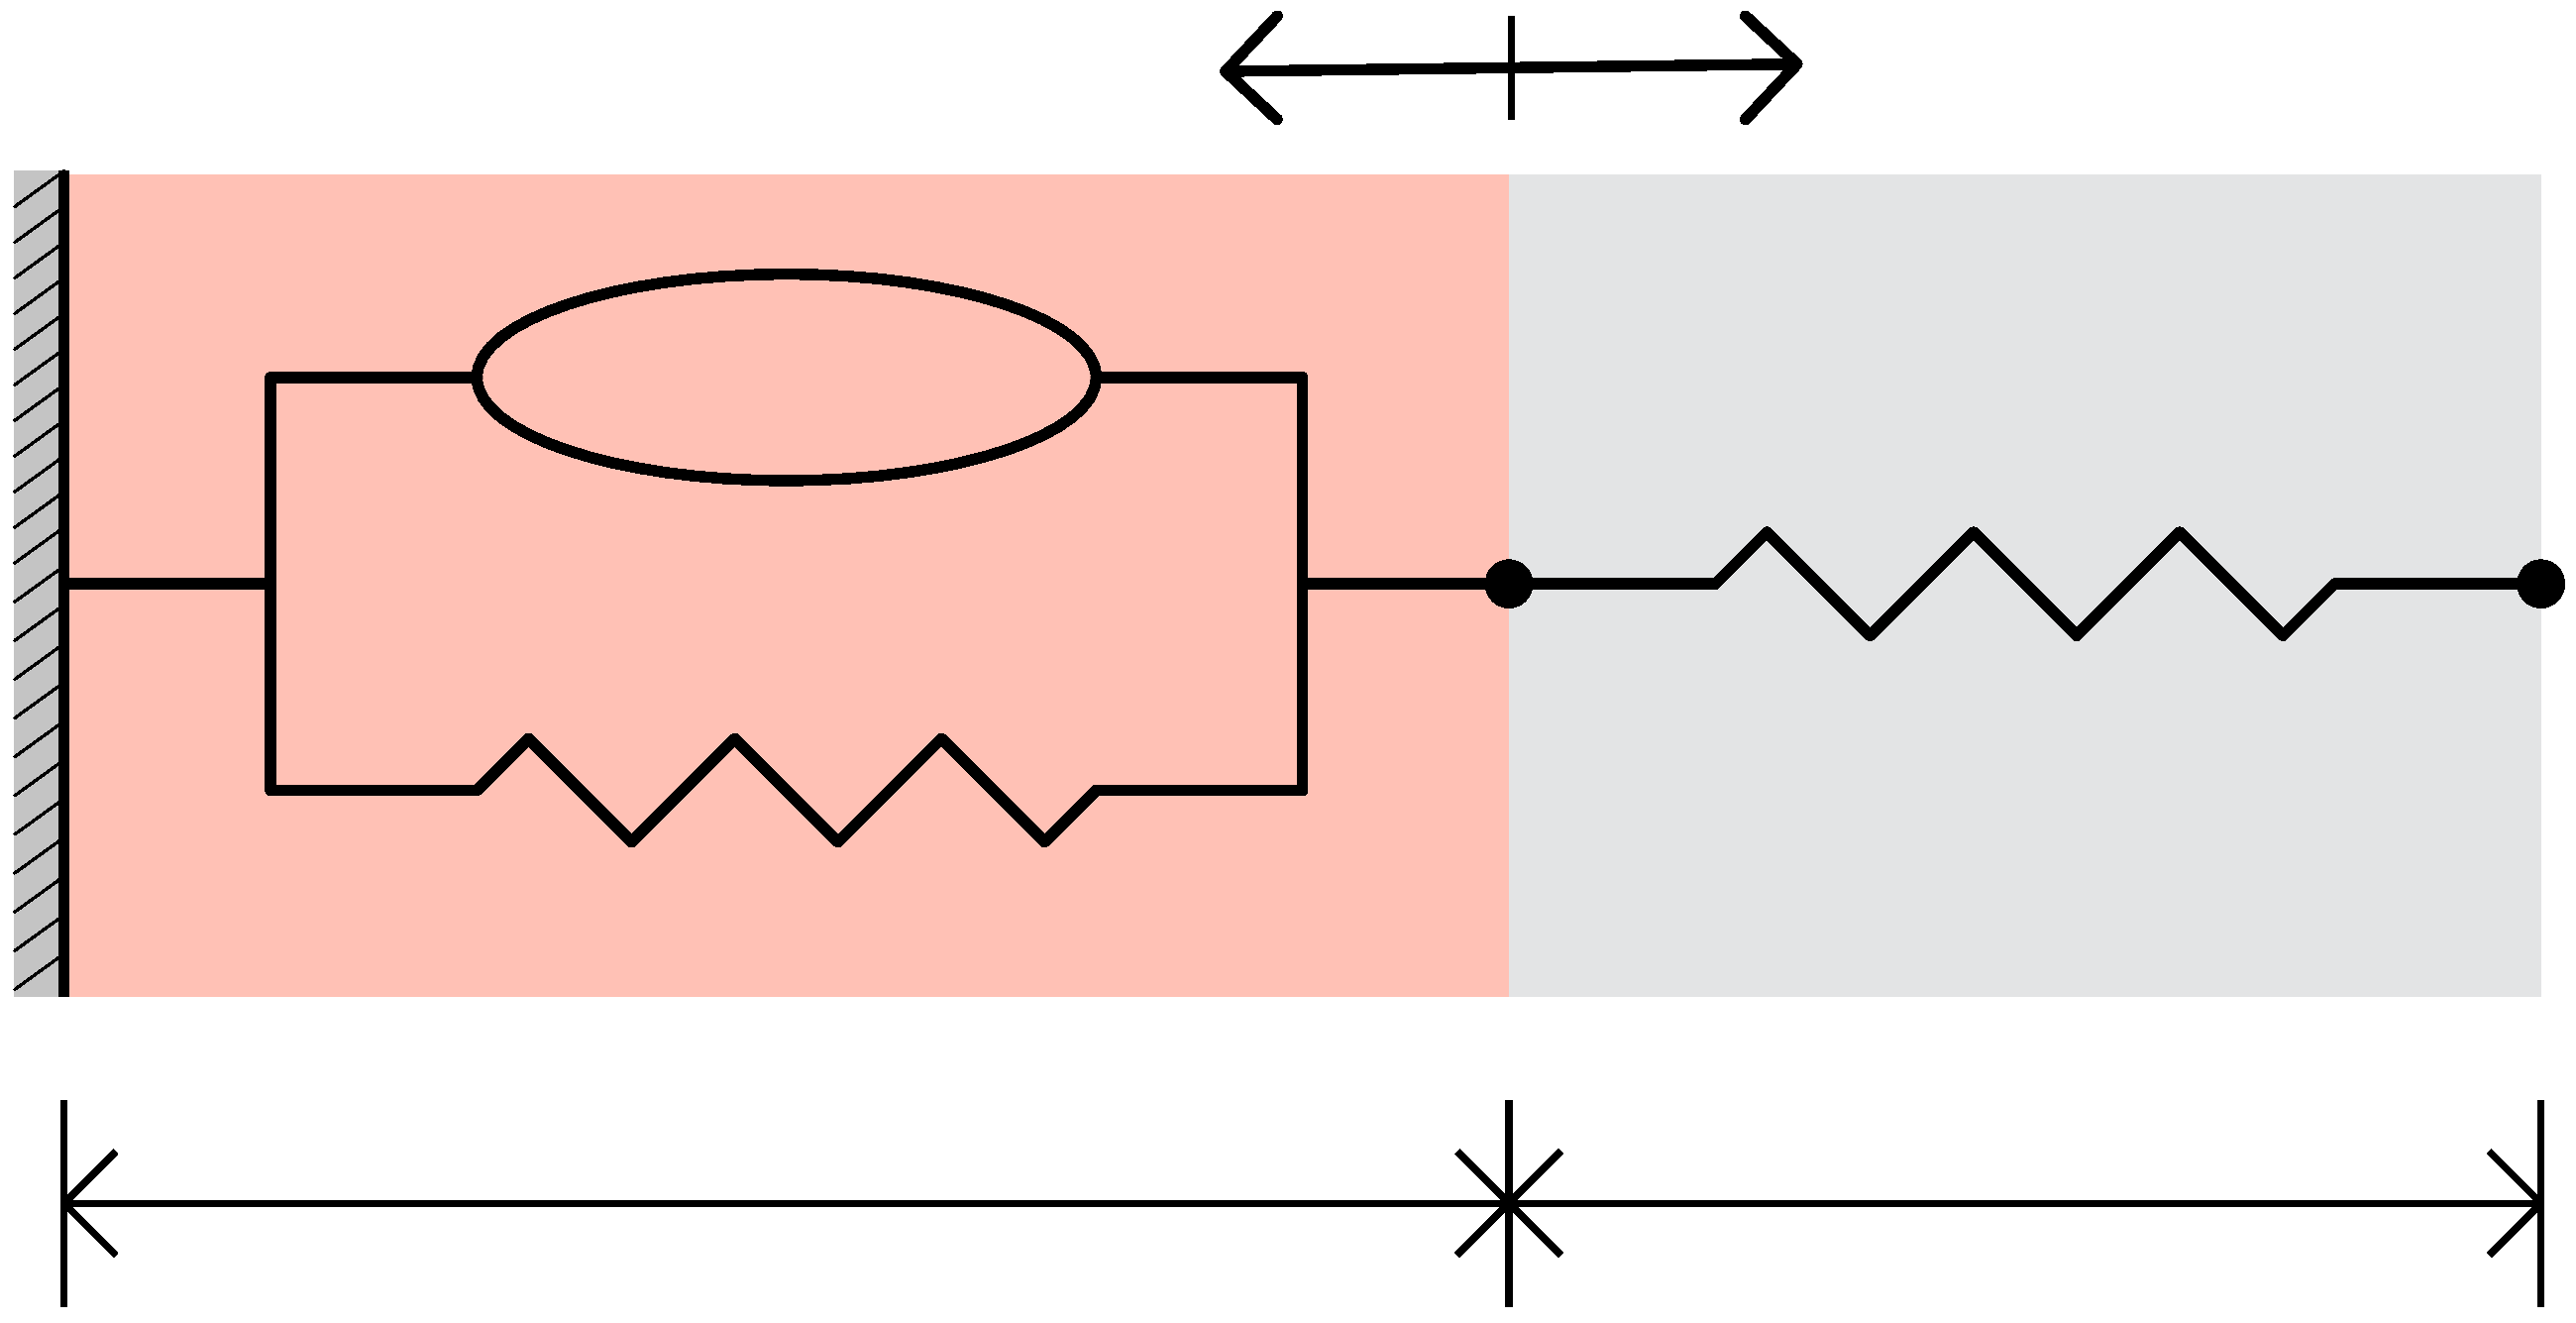
\includegraphics[width=0.3\textwidth]{hill-massless.eps}};
        \node at (-0.92,0.5) {\footnotesize CE};
        \node at (-0.92, -0.47) {\footnotesize PEE};
        \node at (1.33,-0.2) {SEE};
        \node at (-0.92, -1.25) {\footnotesize $L_M$};
        \node at (1.33, -1.25) {\footnotesize $L_T$};
        \node at (0.1, 1.45) {\footnotesize $\vec{F}_M$};
        \node at (0.7, 1.45) {\footnotesize $\vec{F}_T$};
    \end{tikzpicture}
    \hspace{0.5em}
    \begin{tikzpicture}
        \centering
        \node at (-4.5,1) {\huge \textbf{B}};
        \node[inner sep=0pt] at (0,0)
            {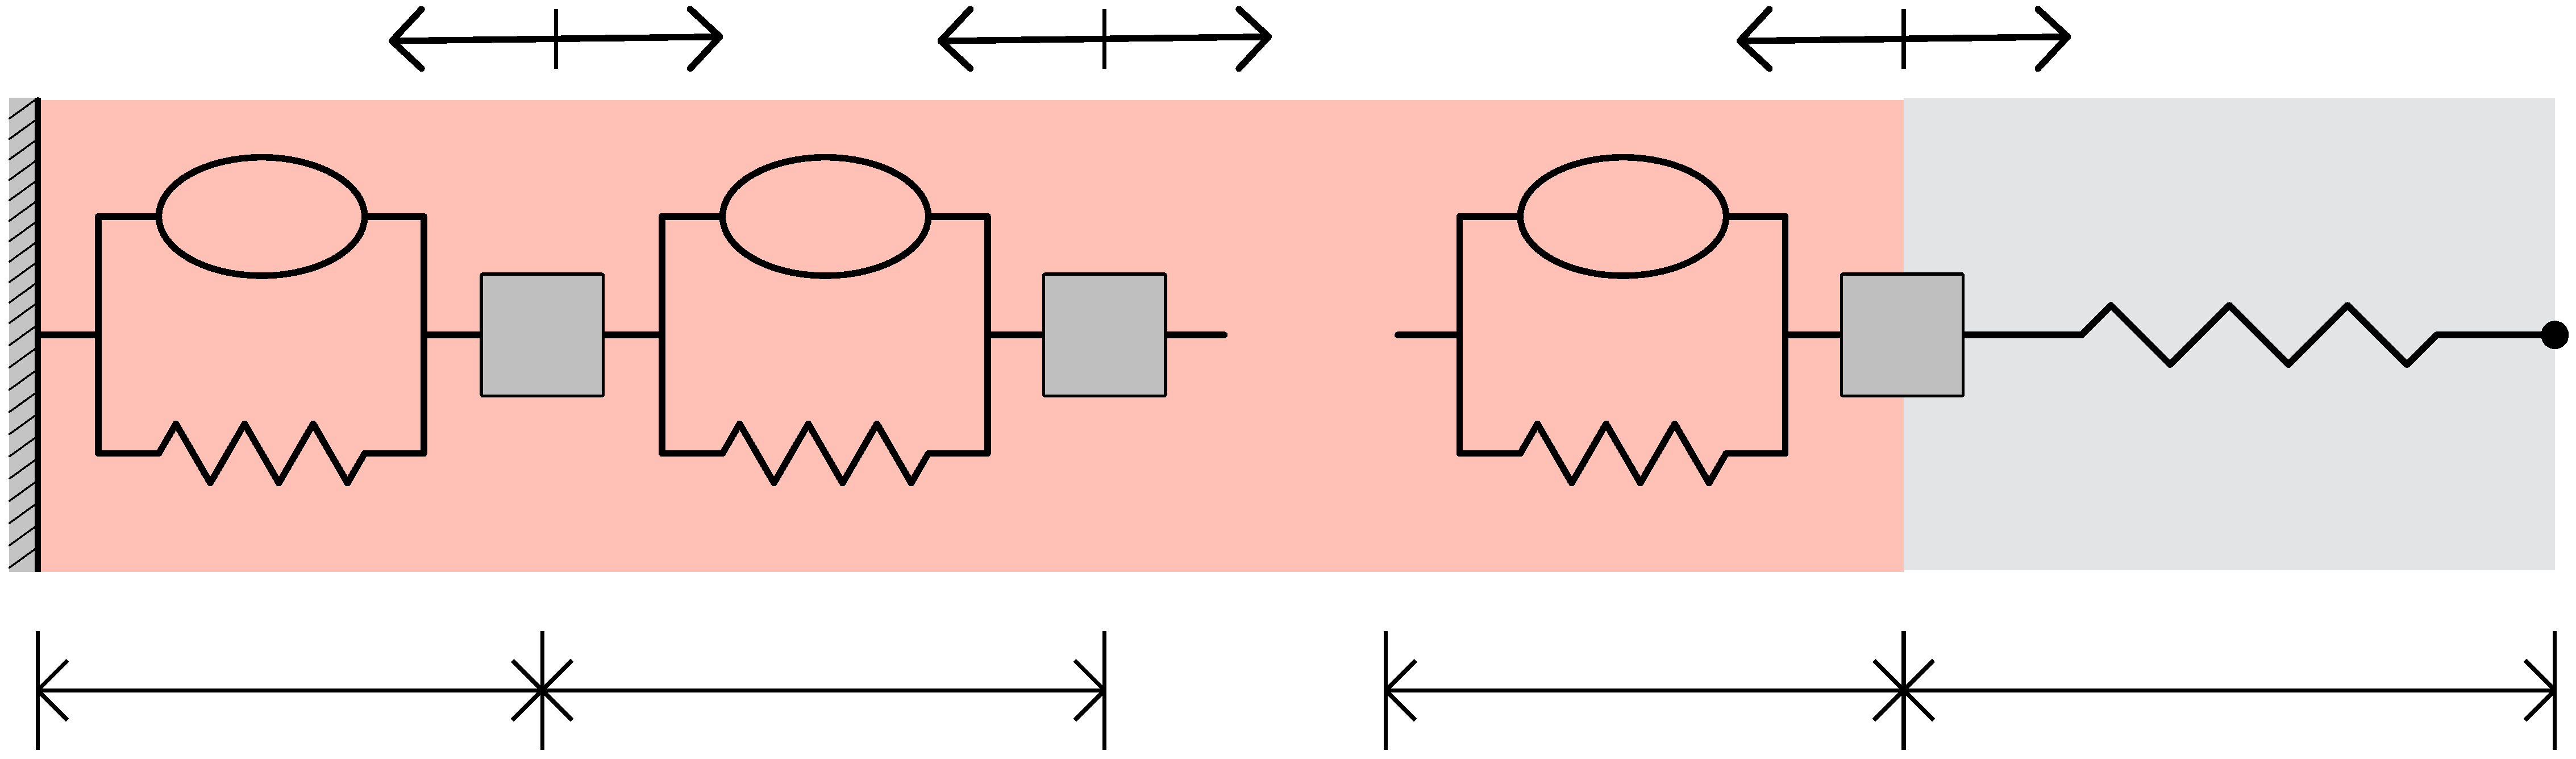
\includegraphics[width=0.525\textwidth]{hill-mass-enhanced.eps}};
        \node at (-2.31, 0.1) {\tiny $m_1$};
        \node at (-0.56, 0.1) {\tiny $m_2$};
        \node at (1.94, 0.1) {\tiny $m_{\hspace{-0.15em}N}$};
        \node at (-3.2, 0.5) {\tiny CE$_1$};
        \node at (-3.2, -0.5) {\tiny PEE$_1$};
        \node at (-3.2, -1.26) {\footnotesize $l_1$};
        \node at (-1.45, 0.5) {\tiny CE$_2$};
        \node at (-1.45, -0.5) {\tiny PEE$_2$};
        \node at (-1.45, -1.26) {\footnotesize $l_2$};
        \node at (1.08, 0.5) {\tiny CE$_{\hspace{-0.15em}N}$};
        \node at (1.08, -0.5) {\tiny PEE$_{\hspace{-0.15em}N}$};
        \node at (1.08, -1.26) {\footnotesize $l_N$};
        \node at (3.05, -0.2) {\tiny SEE};
        \node at (3.05, -1.26) {\footnotesize $L_T$};
        \node at (-2.6, 1.45) {\footnotesize $\vec{F}_1$};
        \node at (-2.0, 1.45) {\footnotesize $\vec{F}_2$};
        \node at (-0.9, 1.45) {\footnotesize $\vec{F}_2$};
        \node at (-0.3, 1.45) {\footnotesize $\vec{F}_3$};
        \node at (1.65, 1.45) {\footnotesize $\vec{F}_N$};
        \node at (2.25, 1.45) {\footnotesize $\vec{F}_T$};
        \node at (0.1,0.14) {\footnotesize $\dots$};
        \node at (-0.1,-1.0) {\footnotesize $\dots$};
    \end{tikzpicture}
    \caption{(A) A simple Hill-type model of the MTU (muscle region in pink, tendon region in grey) using massless springs. Depicted here are the (active) contractile element (CE), the passive elastic element (PEE), and the series elastic element (SEE) representing the tendon. (B) A multi-body mode of the MTU that does not neglect the mass of the muscle, which is equally distributed throughout the muscle segment.}
    \label{fig:muscle_models_1D}
\end{figure}

%\begin{circuitikz}
    %ground
    %\pattern[pattern=north east lines] (0,0) rectangle (7,.25);
    %\draw[thick] (0,.25) -- (7,.25);
    
    %\draw (3,.25) to[spring, l=$k$] (3,2);
    %\draw (4,.25) to[damper, l_=$b$] (4,2);
    %\draw[fill=gray!40] (2.5,2) rectangle (4.5,3);
    %\node at (3.5,2.5) {$m$};
    
    %\draw[thick, ->] (3.5,4) -- (3.5,3);
    %\node at (3.75,3.75) {$F$};   
%\end{circuitikz}

%\begin{circuitikz}
    
    %\pattern[pattern=north east lines] (0,0) rectangle (0.2, 2);
    %\draw[thick] (0.2, 0) -- (0.2, 2);
    %\draw (0.2, 1) -- (0.8, 1);
    %\draw (0.8, 1) -- (0.8, 1.5) -- (1.3, 1.5);
    %\draw (1.9, 1.5) ellipse (6mm and 3mm);
    %\draw (2.5, 1.5) -- (3.0, 1.5);
    %\draw (0.8, 1) -- (0.8, 0.5) -- (1.0, 0.5);
    %\draw (1.0, 0.5) to[R] ++(1.8, 0) -- (3.0, 0.5);
    %\draw (3.0, 0.5) -- (3.0, 1.5);
    %\draw (3.0, 1.0) -- (3.6, 1.0);

%\end{circuitikz}

Equation \eqref{eq:massless_model} (which we refer to as the \textit{massless} model) represents a model of the MTU in which the mass of the muscle is not taken into consideration. While this may seem like an outrageous simplification of the problem, this is actually considered the ``gold-standard'' in muscle modelling. Hence, \textbf{this model's absence of mass (and therefore inertial forces) raises the question of whether including mass has any effect in the prediction of the dynamics (including forces) of the system}. In an attempt to answer this, Chen \cite{EvanThesis} has put forward a muscle model in which the mass of the muscle is equally distributed into $N$ segments (see Figure \ref{fig:muscle_models_1D}B). The dynamics in this model (which we refer to as the \textit{mass-enhanced} model) are given by the set of second-order ODEs:
\begin{subequations} \label{eq:massenhanced_model}
    \begin{align}
        m_1 \ddot{u}_1 &= F_2(\lambda_2, \depsilon_2) - F_1(\lambda_1, \depsilon_1), \\
        m_2 \ddot{u}_2 &= F_3(\lambda_3, \depsilon_3) - F_2(\lambda_2, \depsilon_2), \\
        &\hspace{0.6em} \vdots \notag \\
        m_N \ddot{u}_N &= F_T(\lambda_T) - F_N(\lambda_N, \depsilon_N).
    \end{align}
\end{subequations}
Here, $u_i$ is the displacement of the $i$-th segment, that is,
\begin{equation}
    x_i = u_i + x_i^0, \quad i=1,\dots,N,
\end{equation}
where $x_i^0$ is the initial position of the $i$-th segment. The segment stretches and strain rates, i.e.
\[
\lambda_i = \dfrac{l_i}{l_s^{opt}} = \dfrac{l_i}{l_{mus}^{opt}/N}, \quad \depsilon_i = \dfrac{\dot{\lambda_i}}{\depsilon_0}, \quad i = 1,\dots,N,
\]
can be written in terms of the displacements $u_i$ as
\begin{equation}
    \lambda_1 = \dfrac{u_1 + l_s^0}{l_s^{opt}}, \quad \lambda_2 = \dfrac{u_2-u_1 + l_s^0}{l_s^{opt}}, \quad \dots \quad, \lambda_N = \dfrac{u_N-u_{N-1} + l_s^0}{l_s^{opt}},
\end{equation}
and
\begin{equation}
    \depsilon_1 = \dfrac{\dot{u}_1}{l_s^{opt} \depsilon_0}, \quad \depsilon_2 = \dfrac{\dot{u}_2-\dot{u}_1}{l_s^{opt} \depsilon_0}, \quad \dots \quad, \depsilon_N = \dfrac{\dot{u}_N - \dot{x}_{N-1}}{l_s^{opt} \depsilon_0},
\end{equation}
with $l_s^0 := L_M(0)/N$ is the initial length of each segment.



\section{Biomechanical data and initial conditions}

To compare the performance of the muscle models \eqref{eq:massless_model} and \eqref{eq:massenhanced_model}, we use the motion-capture and electromyography (EMG) data collected in \cite{EvanThesis}. The data corresponds to the human muscle-tendon unit dynamics of three muscles (medial gastrocnemius (MG), vastus medialis (VM), and semitendinosus (ST)) during three tasks (walking, cycling, and running). In particular, we are given to as a set of traces of muscle excitation $\widehat{u}$ and MTU length $L$ over the span of 24.99 seconds.

TO DO HERE

\begin{enumerate}
    \item Explain subject data (mass, height, tasks).
    \item Explain how muscle volume is computed.
    \item initial conditions (either refer to Appendix A or bring those contents here).
\end{enumerate}

\section{Main results}











\chapter{Physiological stability of multi-body models}

Show that the mass enhanced muscle model yields a 1D PDE. Augment the PDE with a Neo-Hookean term. Bring back the PDE to a system of ODEs and show that this model is physiologically stable.
Github repository: derived from mass-enhanced-muscle-model -> separate repository?

\medskip

TITIN -> can we get a FL curve for this or do we have to resort to more intricate implementations?


\chapter{First order is enough: time discretization alternatives for dynamic Neo-Hookean deformation}

Newmark methods, Rothe's vs. method of lines comparisons. Stiff solvers is (one of) the key mathematical concepts here.
Github repository: one-dimensional-muscle-models

\part{Three-dimensional elastodynamics}

\chapter{A Lagrangian framework for a model of skeletal muscle tissue}

Sections to include:
\begin{enumerate}
    \item Lagrangian model
    \item Fully-implicit time discretization
    \item Linearization strategies
\end{enumerate}

\chapter{Flexodeal: a new finite-element tool for studying musculoskeletal dynamics}

\begin{enumerate}
    \item Implementation details
    \item Convergence
    \item Nonlinear Solvers
    \item Different muscle architectures (e.g. bi-pennate)
\end{enumerate}

\chapter{Gearing in muscle tissues: a first-of-its-kind computational study}

From paper w/ James. Add different pennations. Cedar access?



\chapter{Conclusions and future work}


%   BACK MATTER  %%%%%%%%%%%%%%%%%%%%%%%%%%%%%%%%%%%%%%%%%%%%%%%%%%%%%%%%%%%%%%
%
%   References and appendices. Appendices come after the bibliography and
%   should be in the order that they are referred to in the text.
%
%   If you include figures, etc. in an appendix, be sure to use
%
%       \caption[]{...}
%
%   to make sure they are not listed in the List of Figures.
%

\backmatter%
    \addtoToC{Bibliography}
    \bibliographystyle{siam}
    \bibliography{references}

\begin{appendices} % optional

\chapter{Calibration of optimal and initial muscle parameters in the context of experimental data}
\label{app:calibration_optimal_initial_values}

This is from Evan's thesis and the report TR2023-04. Needs to be updated to the appropriate notation.

To minimize overshooting at the beginning of the simulation due to potential imbalance of forces, we must first calibrate our model. The idea is that a system that starts at rest should remain at rest if the initial length of the elements corresponds to their optimal length (in this case, $\widehat{\lambda}_i = 1$). Moreover, the sum of forces should also be zero at the beginning of the simulation. This affects the optimal and initial lengths, respectively, of the muscle belly and tendon.


Let $r$ denote the \textit{estimated} ratio between the length of the muscle belly and the length of the MTU. Then, we can \textit{estimate} the optimal muscle belly and tendon length as follows:
\[
	\widetilde{l_{mus}^{opt}} := l_{MTU}^{opt} r, \qquad \widetilde{l_{ten}^{opt}} := l_{MTU}^{opt}(1-r).
\]
First, in a situation where the MTU is resting at optimal length, the muscle and tendon forces should balance: $F_M(1) = F_T(1)$. However, because there might be discrepancy between the normalization factors used to construct the force-length relationships and the ones used in this work, we assume that the true optimal lengths are small deviations of the estimated ones:
\[
	l_{mus}^{opt} = \widetilde{l_{mus}^{opt}} + \Delta l^{opt}, \qquad l_{ten}^{opt} = \widetilde{l_{ten}^{opt}} - \Delta l^{opt}.
\]
The correction $\Delta l^{opt}$ can then be found by solving the equation
\begin{equation}
	F_P\left( \dfrac{\widetilde{l_{mus}^{opt}}}{\widetilde{l_{mus}^{opt}} + \Delta l^{opt}} \right) = F_T \left( \dfrac{\widetilde{l_{ten}^{opt}}}{\widetilde{l_{ten}^{opt}} - \Delta l^{opt}} \right).	
\end{equation}


Similarly, we can estimate the initial muscle belly and tendon lengths:
\[
	\widetilde{l_{mus}^0} := L(0)r, \qquad \widetilde{l_{ten}^0} := L(0)(1-r).
\]
Therefore, the \textit{true} initial muscle belly and tendon lengths is given by
\[
	l_{mus}^0 = \widetilde{l_{mus}^0} - \Delta l^0, \qquad l_{ten}^0 = \widetilde{l_{ten}^0} + \Delta l^0.
\]
The correction in this case is found by solving:
\begin{equation}
	F_M \left( \dfrac{\widetilde{l_{mus}^0} - \Delta l^0}{l_{mus}^{opt}}\right) = F_T \left( \dfrac{\widetilde{l_{ten}^0} + \Delta l^0}{l_{ten}^{opt}}\right).
\end{equation}



\chapter{Force relationships}

Describe in detail force-length and force-velocity relationships in use.
Github repository: force-relationships

\chapter{Strain energies}

Include all strain energies: base material, ecm, cellular material, fat, aponeurosis/tendon.

\end{appendices}
\end{document}
